% --------------------------------------------------------------------------------

\begin{exercise}[26]

Geben Sie eine $\ast$-erfüllbare Menge an, die nicht erfüllbar ist.

\end{exercise}

% --------------------------------------------------------------------------------

\begin{solution}

\phantom{}

Nach Korollar II.3.14 kann es solch eine Menge nicht geben.

\begin{figure}
    \begin{boxedin}
        \begin{center}
            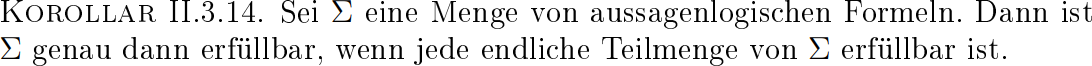
\includegraphics[width = 0.75 \textwidth]{Korollar II.3.14.png} \\
            \vspace{0.5 cm}
            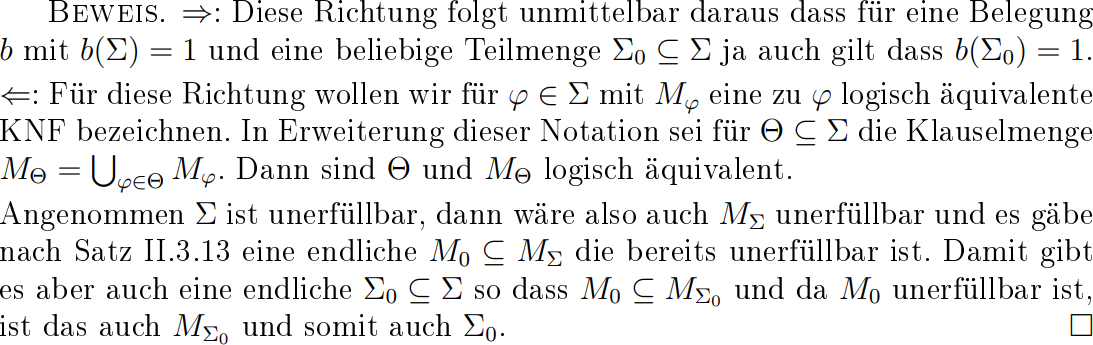
\includegraphics[width = 0.75 \textwidth]{Korollar II.3.14 - Beweis.png}
        \end{center}
    \end{boxedin}
\end{figure}

Sei $\Sigma$ eine unerfüllbare Menge. Für eine beliebige Formel $\varphi \in \Sigma$ definieren wir mit
$M_\varphi$ eine äquivalente KNF. Weiters sei für eine ganze Teilmenge $\Theta \subseteq \Sigma$ die Menge
$M_\Theta := \bigcup_{\varphi \in \Theta} M_\varphi$. Es sei bemerkt, dass $M_\Theta$ erfüllbar ist, genau
dann wenn es eine Belegung gibt, sodass alle $M_\varphi$ erfüllbar sind und das ist genau dann der Fall,
wenn es eine Belegung gibt, sodass $\Theta$ erfüllbar ist. Da $\Sigma$ unerfüllbar ist, gilt das also auch
für $M_\Sigma$. Daher gibt es eine Resolutionswiderlegung $C_1, \dots, C_n$ von $M_\Sigma$. Sei die
endlichen Menge $M_0 \subseteq M_\Sigma$ die Menge aller von der Resolutionswiderlegung verwendeten
Klauseln. Da es für $M_0$ eine Resolutionswiderlegung gibt, ist $M_0$ unerfüllbar.
Da $M_0 \subset M_{\Sigma}$, ist zu jeder Formel $\varphi \in M_0$ die Menge
$\{\psi \in \Sigma: M_{\psi} = \varphi\}$ nicht leer. Nach dem Auswahlaxiom gibt es
eine Abbildung $f$ die jedem $\varphi \in M_0$ ein $\psi \in \Sigma$ zuordnet.
Das Bild $f(M_0)$ ist eine endliche Menge, welche aufgrund der Unerfüllbarkeit von $M_0$
ebenso wieder unerfüllbar ist. Daher ist $\Sigma$ nicht *-erfüllbar.

\end{solution}

% --------------------------------------------------------------------------------
